\documentclass[tikz,border=5pt]{standalone}
\usepackage[T1]{fontenc}
\usepackage{lmodern}
\usetikzlibrary{arrows.meta,positioning,fit}
\begin{document}
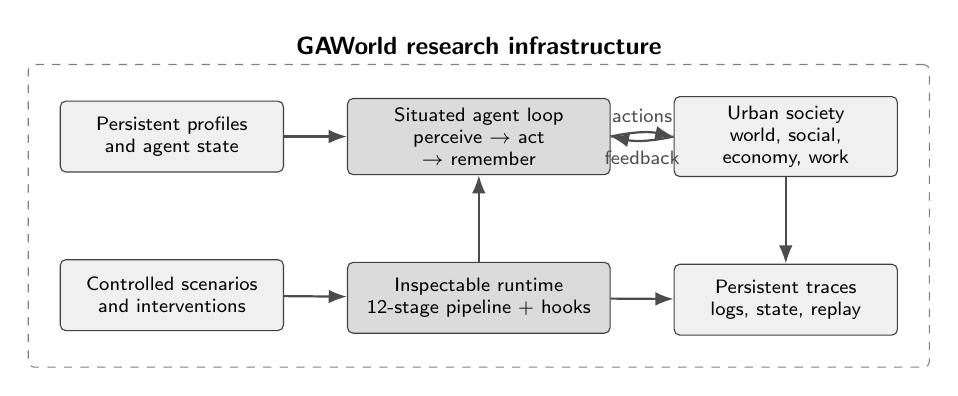
\begin{tikzpicture}[font=\sffamily\scriptsize,>=Latex,
  box/.style={draw=black!75,rounded corners=2pt,fill=black!6,minimum height=9mm,align=center,text width=26mm},
  core/.style={box,fill=black!14,text width=31mm},
  flow/.style={->,thick,black!70}]
\node[box] (profile) {Persistent profiles\\and agent state};
\node[core,right=8mm of profile] (loop) {Situated agent loop\\perceive $\rightarrow$ act\\$\rightarrow$ remember};
\node[box,right=8mm of loop] (society) {Urban society\\world, social, economy, work};
\draw[flow] (profile) -- (loop);
\draw[flow] (loop.east) to[bend left=12] node[above]{actions} (society.west);
\draw[flow] (society.west) to[bend left=12] node[below]{feedback} (loop.east);

\node[box,below=11mm of profile] (experiments) {Controlled scenarios\\and interventions};
\node[core,below=11mm of loop] (runtime) {Inspectable runtime\\12-stage pipeline + hooks};
\node[box,below=11mm of society] (traces) {Persistent traces\\logs, state, replay};
\draw[flow] (experiments) -- (runtime);
\draw[flow] (runtime) -- (traces);
\draw[flow] (runtime) -- (loop);
\draw[flow] (society) -- (traces);

\node[draw=black!50,dashed,rounded corners=2pt,fit=(profile)(society)(experiments)(traces),
      inner sep=4mm,label={[font=\sffamily\bfseries\small]above:GAWorld research infrastructure}] {};
\end{tikzpicture}
\end{document}
